%%%%%%%%%%%%%%%%%%%%%%%%
%% Sample use of the infthesis class to prepare a thesis. This can be used as 
%% a template to produce your own thesis.
%%
%% The title, abstract and so on are taken from Martin Reddy's csthesis class
%% documentation.
%%
%% MEF, October 2002
%%%%%%%%%%%%%%%%%%%%%%%%

%%%%
%% Load the class. Put any options that you want here (see the documentation
%% for the list of options). The following are samples for each type of
%% thesis:
%%
%% Note: you can also specify any of the following options:
%%  logo: put a University of Edinburgh logo onto the title page
%%  frontabs: put the abstract onto the title page
%%  deptreport: produce a title page that fits into a Computer Science
%%      departmental cover [not sure if this actually works]
%%  singlespacing, fullspacing, doublespacing: choose line spacing
%%  oneside, twoside: specify a one-sided or two-sided thesis
%%  10pt, 11pt, 12pt: choose a font size
%%  centrechapter, leftchapter, rightchapter: alignment of chapter headings
%%  sansheadings, normalheadings: headings and captions in sans-serif
%%      (default) or in the same font as the rest of the thesis
%%  [no]listsintoc: put list of figures/tables in table of contents (default:
%%      not)
%%  romanprepages, plainprepages: number the preliminary pages with Roman
%%      numerals (default) or consecutively with the rest of the thesis
%%  parskip: don't indent paragraphs, put a blank line between instead
%%  abbrevs: define a list of useful abbreviations (see documentation)
%%  draft: produce a single-spaced, double-sided thesis with narrow margins
%%
%% For a PhD thesis -- you must also specify a research institute:
% \documentclass[phd,ilcc,twoside]{infthesis}

%% For an MPhil thesis -- also needs an institute
% \documentclass[mphil,ianc]{infthesis}

%% MSc by Research, which also needs an institute
% \documentclass[mscres,irr]{infthesis}

%% Taught MSc -- specify a particular degree instead. If none is specified,
%% "MSc in Informatics" is used.
\documentclass[msc,ai,deptreport,twoside]{infthesis}
% \documentclass[msc]{infthesis}  % for the MSc in Informatics

%% Master of Informatics (5 year degree)
% \documentclass[minf]{infthesis}

%% Undergraduate project -- specify the degree course and project type
%% separately
% \documentclass[bsc]{infthesis}
% \course{Artificial Intelligence and Psychology}
% \project{Fourth Year Project Report}

%% Put any \usepackage commands you want to use right here; the following is 
%% an example:
\usepackage{natbib}
\usepackage{breakcites}
\usepackage{amsmath}
\usepackage{graphicx}
\usepackage{tikz}
\usepackage{algorithm}
\usepackage[noend]{algpseudocode}

%% Information about the title, etc.
\title{Effective Grammatical Error Correction with Neural Machine Translation Techniques}
\author{Shubha Guha}

%% If the year of submission is not the current year, uncomment this line and 
%% specify it here:
% \submityear{1785}

%% Optionally, specify the graduation month and year:
% \graduationdate{February 1786}

%% Specify the abstract here.
\abstract{
This thesis presents the results of applying neural machine translation techniques with a novel objective function adapted to the task of grammatical error correction. It demonstrates that placing more importance on grammatical errors than on grammatically correct text during training succeeds in forcing neural machine translation systems to learn more effectively to correct errors rather than to copy incorrect writing. More specifically, the use of an edit-based weighted token-level cost function dramatically improves recall as hoped, without compromising precision whatsoever.
}

%% Now we start with the actual document.
\begin{document}

%% First, the preliminary pages
\begin{preliminary}

%% This creates the title page
\maketitle

%% Acknowledgements
\begin{acknowledgements}
Heartfelt thanks to my supervisor, Dr. Kenneth Heafield, who has never failed to encourage fun. He has been an accessible mentor, on project business and besides, a source of knowledge, experience, and guidance as well as positivity throughout this project. Also thanks to Roman Grundkiewicz who fielded many questions and provided scripts and data.

I thank my father, Angshuman Guha, for his eager mentorship and willing ears at any hour, and my mother, Atreyee Guha, for her tenacious confidence in me.

I owe a deep gratitude to the companions who have carried my spirits throughout this year and who have inspired me to learn and thrive in both dark times and bright.
\end{acknowledgements}

%% Next we need to have the declaration.
\standarddeclaration

%% Finally, a dedication (this is optional -- uncomment the following line if
%% you want one).
% \dedication{To my mummy.}

%% Create the table of contents
\tableofcontents

%% If you want a list of figures or tables, uncomment the appropriate line(s)
% \listoffigures
% \listoftables

\end{preliminary}

%%%%%%%%
%% Include your chapter files here. See the sample chapter file for the basic
%% format.

\chapter{Introduction} \label{ch:intro}
% objective
Grammatical error correction (GEC) is the task of automatically transforming text with potential grammatical errors into grammatically correct text. Although both input and output text are in the same language, this transformation is similar to the task of translating text from one language to another, so much of recent work has focused on applying the same techniques to GEC that have been successful for translation. While neural machine translation (NMT) techniques have generally outperformed statistical machine translation (SMT) techniques at translation tasks, the same pattern has not been the case for GEC. GEC systems trained using standard NMT methods tend to have low recall, i.e. they learn to copy instead of correcting grammatical errors; consequently, SMT systems remain more effective for GEC. The goal of this project is to improve recall using NMT for GEC.

% motivation
A key difference that sets apart GEC from MT is that part or all of the input text can be identical to the corresponding output text; not only are both texts in the same language but most input text is error-free in practice (see section \ref{subsec:error-rates} for frequency of grammatical errors in commonly used GEC datasets). An unfortunate consequence is that out-of-the-box NMT techniques result in GEC systems that learn to copy instead of correcting grammatical errors, resulting in poor recall. Perhaps this issue has been neglected in recent research due to the fact that the standard metric for the past few years is an $F_{0.5}$ score, which places twice the importance on precision as on recall; the idea behind it is that producing output that is unchanged and equally ungrammatical to the input is preferable to producing output that is changed and more ungrammatical. In this project we focus particularly on recall instead of this $F_{0.5}$ score. We hypothesise that applying a higher cost to grammatical errors during training will prevent the system from learning to copy and will improve its recall.

% results
After modifying the default training objective to relatively punish missed grammatical errors more than unnecessary edits, we successfully forced several models to learn to correct grammatical errors. In general, the greater the relative emphasis, the greater the improvement in recall. As an added bonus, we found that far from sacrificing any precision, our approach ended up improving it as well, proving our strategy an unequivocal success.

% outline
% TODO: revisit
The remainder of this document is as follows: Chapter \ref{ch:background} surveys the evolution of recent GEC work, including the development of the task-specific MaxMatch scoring framework. It outlines the methods of phrase-based SMT and NMT and reviews work that has applied these approaches to GEC. Chapter \ref{ch:methods} summarises the model architecture used in all of our experiments; training hyperparameter values, the original and modified objective function, convergence criterion, and tools used; as well as the datasets used in this work. Chapter \ref{ch:results} compares the results of baseline models against models with varying values of the novel training hyperparameter. Finally, chapter \ref{ch:conclusion} concludes with further observations and suggestions for future work.
\chapter{Background} \label{ch:background}
As described in the research proposal for this project, several GEC shared tasks at the beginning of this decade led to significant advances in research: the Helping Our Own (HOO) shared tasks in 2011 and 2012 \citep{Dale2011HelpingTask, Dale2012HOOTask}, and the shared tasks at the 17th and 18th conferences on Computational Natural Language Learning (CoNLL) in 2013 and 2014 \citep{Ng2013TheCorrection, Ng2014TheCorrection}. In this timeframe, a new task-specific scoring framework was developed \citep{Dahlmeier2012BetterCorrection} and the spotlight shifted from highly linguistically motivated and error-specific classifiers and rule-based methods to more generalized machine translation techniques. Error-specific approaches, while they require more linguistic expertise and model complexity to achieve full coverage of grammatical error types, have the advantage of performing particularly well on the specific error types they target. On the other hand, statistical machine translation (SMT) methods have achieved state-of-the-art results on GEC, capturing complex interactions between different error types without requiring the individual construction of as many component models. Some have even attempted to combine the advantages of each technique with hybrid systems \citep{Susanto2014SystemCorrection,Rozovskaya2016GrammaticalClassifiers}.

Meanwhile, machine translation (MT) has experienced its own revolution, from the advent of neural machine translation (NMT) methods around 2013 and 2014 \citep{Kalchbrenner2013RecurrentModels,Cho2014LearningTranslation,Cho2014OnApproaches,Sutskever2014SequenceNetworks} to their adoption by Google and Microsoft last year \citep{Wu2016GooglesTranslation}. While many GEC researchers have continued to improve the performance of phrase-based SMT \citep{Junczys-Dowmunt2016Phrase-basedCorrection,Chollampatt2016NeuralCorrection} and hybrid classifier-SMT systems \citep{Susanto2014SystemCorrection,Rozovskaya2016GrammaticalClassifiers}, those pioneering the application of NMT methods to GEC \citep{Xie2016NeuralAttention,Yuan2016GrammaticalTranslation} have not been able to meet the state-of-the-art performance according to the accepted scoring method using the MaxMatch scoring framework, presented in the next section.

\section{MaxMatch Scorer}
Establishing a standard evaluation metric is key to building on prior work and making progress on any research topic. The way that GEC systems have been evaluated in most recent work can be broken down to two components: first, a method to align a pair of sentences and extract the edits necessary to transform the given input to the given output; second, a scoring function based on Levenshtein edit operations (insertion, deletion, and substitution) to assess the accuracy of the transformation, typically an $F$ score between the extracted edits and a set of gold standard edits.

\subsection{Alignment}
% TODO: alignment problem vs scoring function, why is alignment an important task?
There is often more than one way to align two sentences and identify a set of edits that represent their differences. There can be more than one possible set of token-level edits leading to the same resulting sentence, but there can also be phrase-level edits on top of these, resulting in some ambiguity around which system edits to feed into the scoring function.

\citet{Dahlmeier2012BetterCorrection} illustrate the problem with an example from the 2011 HOO shared task:

\begin{table}[h]
\centering
\begin{tabular}{ r l }
\tabularnewline \hline \hline
Source & Our baseline system feeds word into PB-SMT pipeline. \\
Hypothesis & Our baseline system feeds \textbf{a} word into PB-SMT pipeline. \\
\hline
\end{tabular}
\caption{Example of ambiguous edit extraction from HOO 2011: is the edit an insertion of the token \texttt{a}, the substitution of the token \texttt{word} with the phrase \texttt{a word}, or something else?}
\label{tab:maxmatch-hoo-2011-example}
\end{table}

The official evaluation script of the shared task extracts the edit $\epsilon \rightarrow \texttt{a}$, while the gold standard annotation is $\texttt{word} \rightarrow \texttt{\{a word, words\}}$. Even though both edits could produce the same output string, there is no overlap between the extracted system edit and the gold standard edit choices, so the hypothesis is considered incorrect.

% However, identifying system edits from a pair of input and output texts proved ambiguous in cases where a proposed edit resulted in the correct output string but did not correspond to an edit in the gold standard set. For example, given an input sentence, ``I'm craving burger,'' and system output, ``I'm craving a burger,'' if the gold standard edits were $\texttt{burger} \rightarrow \texttt{\{a burger, burgers\}}$, the HOO scorer would deterministically extract as a system edit $\epsilon \rightarrow \texttt{a}$ (insertion of the word `a') regardless of the gold standard edits. Even though the results of the proposed system edit and of one of the gold standard choices are the same, the HOO evaluation framework would underestimate the system's performance.

To solve this problem, \citet{Dahlmeier2012BetterCorrection} designed the MaxMatch ($M^2$) scoring system to choose from ambiguous system edit possibilities in order to maximize the overlap between system and gold standard edits. The $M^2$ scorer first constructs an edit lattice by filling in a matrix with the Levenshtein distances between substrings of the tokenised input and output and computing all shortest paths through the matrix that transform the input sentence into the system output. Table \ref{tab:maxmatch-levenshtein-matrix} depicts the Levenshtein matrix between source \texttt{i studying informatic .} and hypothesis \texttt{i am studying informatics .}

\begin{table}[h]
\centering
\begin{tabular}{|r|c|c|c|c|c|c|}
\hline
 &  & i & am & studying & informatics & . \\ \hline
 & 0 & 1 & 2 & 3 & 4 & 5 \\ \hline
i & 1 & 0 & 1 & 2 & 3 & 4 \\ \hline
studying & 2 & 1 & 1 & 1 & 2 & 3 \\ \hline
informatic & 3 & 2 & 2 & 2 & 2 & 3 \\ \hline
. & 4 & 3 & 3 & 3 & 3 & 2 \\ \hline
\end{tabular}
\caption{Levenshtein matrix between \texttt{i studying informatic .} and \texttt{i am studying informatics .}}
\label{tab:maxmatch-levenshtein-matrix}
\end{table}

The shortest paths are represented as a graph with each node corresponding to a cell from the Levenshtein matrix and each edge corresponding to an edit operation: insertion, deletion, substitution, or no change. Since GEC data annotations sometimes include phrase-level like $\texttt{studying} \rightarrow \texttt{am studying}$ for the example above, the alignment framework should also allow some phrase-level edits in which some words remain unchanged. However, it should do so within reason, without allowing edits spanning long sequences in which many words remain unchanged, so the number of permitted unchanged words in an edit is limited by a parameter (a reasonable default is 2). These additional edits are added to the edit lattice as new edges that combine adjacent existing edges, as illustrated in \ref{fig:maxmatch-edit-lattice}.

\tikzstyle{unit}=[circle, minimum size=1.2cm, draw=black, inner sep=0pt]

\begin{figure}[h]
\centering
  \begin{tikzpicture}[el/.style = {inner sep=2pt, align=left, sloped}, every label/.append style = {font=\footnotesize}]
    \matrix[row sep=1cm,column sep=1.3cm] {
      \node (0) [unit] {(0,0)}; &
      \node (1) [unit] {(1,1)}; &
      \node (2) [unit] {(1,2)}; &
      \node (3) [unit] {(2,3)}; &
      \node (4) [unit] {(3,4)}; &
      \node (5) [unit] {(4,5)};\\
    };
    
    \path[->]
    (0) edge node[el,above,yshift=10] {\texttt{i}} (1)
    (1) edge node[el,above,yshift=10] {\texttt{am}} (2)
    (1) edge [bend right=40] node[el,below,yshift=-10] {\texttt{studying/am studying}} (3)
    (2) edge node[el,above,yshift=15] {\texttt{studying}} (3)
    (3) edge node[el,below,yshift=50] {\texttt{informatic/}\\\texttt{informatics}} (4)
    (4) edge node[el,above,yshift=10] {\texttt{.}} (5);
  \end{tikzpicture}
\caption{Edit lattice from source \texttt{i studying informatic .} to hypothesis \texttt{i am studying informatics .}}
\label{fig:maxmatch-edit-lattice}
\end{figure}

\subsection{Edit Extraction}
Based on this edit lattice, the $M^2$ scorer chooses the complete set of edits from input to output which maximally match the set of gold standard edits. Matches are defined as any edit with the same start and end position in the input sentence and with proposed correction included in the gold standard correction.

\subsection{Scoring Function}
Initially, GEC researchers continued using $F_1$ as the scoring function with the results of $M^2$ alignment and edit extraction, but beginning with CoNLL-2014, it became standard to use the $F_{0.5}$ score (for reasons mentioned in chapter \ref{ch:intro}), and $M^2$ score became synonymous with $M^2$ edit extraction followed by $F_{0.5}$ score.

\section{GEC Approaches}
We can look to the CoNLL shared tasks of 2013 and 2014 to sample the range of possible approaches to GEC. These shared tasks not only popularised the $M^2$ scoring framework but also introduced datasets that would continue to be used commonly in GEC research to this day.

\subsection{Classifiers}
One of the most popular approaches among submissions to CoNLL-2013 was error-specific machine learning classifiers, one for each of the five grammatical error types included in the task. Five of the submissions were systems based on maximum entropy; others used Naive Bayes, SVMs, perceptrons, and other classifiers. The system with the best $F_1$ score on the test set (42.14\%) consisted of a multi-class averaged perceptron for article or determiner errors, and Naive Bayes for the remaining error types (preposition, noun number, verb form, and subject-verb agreement errors).

Machine learning classifiers remained a common approach in the CoNLL-2014 submission, though almost always in combination with other approaches so as to increase coverage of the 28 error types included in the task. The second best $F_{0.5}$ score on the test set (26.79\%), in spite of handling only nine of the 28 error types, was achieved by a system using ``different combinations of averaged perceptron, Naive Bayes, and pattern-based learning trained on different data sets for different error types'' \citep{Ng2014TheCorrection}.

\subsection{Rule-Based}
Four CoNLL-2013 submissions were rule-based classifiers and two hybrid systems included rule-based components in a pipeline with other methods. CoNLL-2014 similarly included rule-based approaches, but usually mixed with other approaches. The highest $F_{0.5}$ score achieved in CoNLL-2014 (37.33\%) was by a system using rule-based classifiers as a first pass, followed by four steps of ranking hypotheses based on language model probabilities, statistical machine translation, LM ranking again, and type filtering. Hand-crafted rules require extensive linguistic domain expertise Needless to say, purely rule-based techniques no longer appear among the best performing GEC systems.

\subsection{Language Models}
As mentioned for the best performing submission to CoNLL-2014, using language model probabilities to rank hypotheses is another approach, often implemented as a component in a more complex system. It conveniently does not require an annotated grammatical error correction corpus to train an n-gram language model, simply a corpus of grammatically correct text. The result is a way of not only possibly generating new grammatical hypotheses but also comparing their correctness to the source sentence to ensure an improvement.

% CoNLL-2013 also introduced the datasets that are commonly used for GEC until today (described more fully in section \ref{sec:datasets}) and 
% The CoNLL shared tasks of 2013 and 2014 popularised the use of the $M^2$ scoring framework and witnessed a range of methods for GEC, much of which came to dominate how GEC research is done today.
% TODO: why do we care? they introduce the datasets (ref section) and there are other approaches besides machine translation (e.g. CoNLL briefly)

% The CoNLL-2013 shared task covered only five grammatical error types: article or determiner errors, preposition errors, noun number errors, verb form errors, and subject-verb agreement errors. The majority of systems built by the sixteen teams who submitted descriptive papers were error-specific classifiers. Some classifiers were trained on examples that encoded the context in which each error type occurred, some used hand-crafted deterministic rules, and some were built with a combination of the two approaches. A handful of systems were built using machine translation approaches, both phrase-based and syntax-based statistical machine translation, and two systems used language modeling to choose a corrected sentence that is more likely than the uncorrected sentence. These different approaches are also used in combination, in some cases set up as a pipeline to handle different error types with different GEC systems.

% The CoNLL-2014 shared task expanded coverage to include all 28 error types annotated in its training dataset (NUCLE, the same training dataset used for CoNLL-2013). Additional error types included verb tense errors, pronoun reference errors, wrong idioms, etc. Including such varied error types that potentially interact in complicated ways made it much harder to approach the task one error type at a time. As a result, there was a greater prevalence of error-agnostic approaches such as language modeling and machine translation (phrase-based only this time, not syntax-based) among the systems implemented by the twelve teams who submitted system description papers. The submission with the best $F_{0.5}$ score used a pipeline of deterministic rules, language model ranking, and SMT.

\section{The Machine Translation Approach}
When CoNLL-2014 increased coverage from five to 28 error types, systems based on error-specific approaches like machine learning and rule-based classifiers became somewhat less practical to build and a larger portion of submissions turned to machine translation techniques, which frame GEC as the translation of ungrammatical text into grammatical text.
% With the 2013 and 2014 CoNLL shared tasks, work in grammatical error correction started shifting more toward machine translation techniques. GEC can be framed as the translation of ungrammatical text into grammatical text.

In this section, we use the usual MT terminology of translating a foreign/source sentence $f$ into an English/target sentence $e$, except in GEC both source and target are in English and the source sentence $f$ may have grammatical errors while the target sentence $e$ has none.

\subsection{Statistical Machine Translation}
The problem of statistical machine translation can be posed using the noisy channel framework and Bayes' Rule as finding the most likely translation $\hat{e}$ for a sentence $f$ in a foreign language:
\begin{equation} \label{eq:bayes}
	\hat{e}=\underset{e}{\arg\!\max}\ p(e|f)=\underset{e}{\arg\!\max}\ p(e)p(f|e)
\end{equation}
This formulation breaks the system down to two components: a language model $p(e)$ and a translation model (or conditional language model) $p(f|e)$. As the probability of a particular sequence of words occurring in a particular order, the language model represents how correct the target sentence is. \citet{Zens2002Phrase-basedTranslation} further breaks down the translation model into a lexicon and an alignment model.

% TODO: delete? who cares about word-based SMT?
In word-based SMT, the translation probability $p(f|e)$ can be represented with an optional sentence length probability, in addition to lexicon probabilities and alignment probabilities:
\begin{equation} \label{eq:word-based}
	p(f|e)=p(J|e)\sum_{a}\prod_{j=1}^{J}[p(f_j|e_{a_j})p(a_j|a_{j-1},I,J)]
\end{equation}
where $J$ and $I$ are the lengths of the source and target sentences $f$ and $e$, respectively, and $a_j$ is the index of the target word aligned to source word $f_j$. The lexicon probability $p(f_j|e_{a_j})$ is the probability that source word $f_j$ translates to target word $e_{a_j}$. The alignment probability $p(a_j|a_{j-1},I,J)$ is the probability that the position of source word $f_j$ maps to the position of target word $e_i$, given the alignments of previous words in the source sentence and the lengths of the source and target sentences.

In phrase-based SMT, the segmentation of the sentence pair into $K$ phrases is an additional hidden variable $B$. Assuming all segmentations have the same probability and allowing only monotone translations:
\begin{equation} \label{eq:phrase-segmentation}
	p(f|e)=\prod_{k=1}^{K}p(f_k|e_k)
\end{equation}
where each phrase translation probability $p(f_k|e_k)$ is estimated by its relative frequency:
\begin{equation} \label{eq:phrase-translation-prob}
	p(f_k|e_k)=\frac{N(f_k,e_k)}{N(e_k)}
\end{equation}
These are counts in the training corpus: $N(e_k)$ is the number of times the phrase $e_k$ occurred, $N(f_k,e_k)$ the number of times $f_k$ appeared as a translation of $e_k$. Once counted (trained), these estimated probabilities are looked up in a phrase translation table for decoding.

Combining Equations \ref{eq:bayes}, \ref{eq:phrase-segmentation}, and \ref{eq:phrase-translation-prob}, as well as a translation model scaling factor $\lambda$ (to indicate relative importance of language model and translation model contributions), the task of monotone translation becomes something more like this:
\begin{equation} \label{eq:stat-mt-summary}
	\hat{e}=\underset{e,B}{\arg\!\max}{\prod_{i=1}^{I}p(e_i|e_1,e_2,...,e_{i-1}) \prod_{k=1}^{K}p(f_k|e_k)^\lambda}
\end{equation}

For non-monotone translations, the task also includes a distance-based phrase reordering (or distortion) probability $d$ \citep{koehn2009statistical}:
\begin{equation} \label{eq:stat-mt-distortion-summary}
	\hat{e}=\underset{e}{\arg\!\max}{\prod_{i=1}^{I}p(e_i|e_{<i})^{\lambda_{LM}} \prod_{k=1}^{K}p(f_k|e_k)^{\lambda_{\phi}}}d(start_i-end_{i-1}-1)^{\lambda_{d}}
\end{equation}
Each feature has a relative weight $\lambda$ that must be learned through training.

% TODO: more features? see statmt/Moses wiki on Scoring Phrases: http://www.statmt.org/moses/?n=FactoredTraining.ScorePhrases

% this is where it starts going wrong
% In \cite{Koehn2003StatisticalTranslation}, there is a third component $\omega^{\texttt{length}(e)}$, where generally $\omega>1$ to bias the system to produce longer output sentences as a way of ``calibrating'' the source and target sentence lengths (much like the standard metric for machine translation, BLEU, penalizes short translations). In phrase-based translation, the translation model (TM) operates at the phrase level such that the probability $p(f|e)$ for the whole sentence can be broken down further:
% \begin{equation}
% 	p(f|e)=\prod_{i=1}^{I}p(f_i|e_i)d(a_i-b_{i-1})
% \end{equation}
% where $I$ is the number of phrases in the segmented foreign sentence $f$, so $f_i$ and $e_i$ are respectively the foreign and English phrases corresponding to the $i$th phrase of the foreign sentence, and $d$ is a distortion model that captures any phrase reordering that should occur as a result of translation.

% decoder, beam search
% training

% \subsubsection{Features} %TODO

\subsubsection{Hybrid Classifier-SMT Systems for GEC}
% Susanto et al. (2014)
\citet{Susanto2014SystemCorrection} surpassed the performance of the best system from CoNLL-2014 using a hybrid system with both error-specific classifiers and SMT. Their best reported $F_{0.5}$ score of 39.39\% on the test data from CoNLL-2014 resulted from a combination of four independent GEC systems: two that were pipelines of classifier-based correction steps of six common error types (spelling errors, noun number errors, preposition errors, punctuation errors, article errors, and verb form or subject-verb agreement errors) and two that were SMT models. The pipeline systems differed in the order of the correction steps (swapped noun number and article errors), and the SMT systems differed in phrase table construction (two phrase tables built from two separate corpora versus one phrase table built from the concatenation of the two corpora). Three of the six correction steps used classifiers learned from context features for noun number, prepositions, and articles; two were rule-based classifiers to fix punctuation errors and subject-verb agreement errors; and the first correction step was the output of an open source spell-checker (Jazzy), whose output was filtered using language model probabilities. Neither individual systems nor combinations of one pipeline and one SMT system each could match the performance of the combination of all four systems. The recall of the four-part system was 19.14\%, but the two pipeline systems achieved 23.99\% and 22.77\% individually

% Rozovskaya & Roth (2016)
More recently, \citet{Rozovskaya2016GrammaticalClassifiers} far surpassed even this performance with a classifier-SMT model combination that scored 47.40\% on the CoNLL-2014 test set (recall of 25.64\%). The classifier used in the final system combination was initially trained on native data, i.e. a corpus of text assumed to be grammatically correct, then ``tailored'' by artificially introducing grammatical error patterns from a learner corpus, and finally further enhanced by introducing mechanical errors in punctuation, spelling, and capitalization. By running the classifier's output through an SMT system trained on the Lang-8 parallel corpus, they pushed the state-of-the-art to 8 percentage points more than \citet{Susanto2014SystemCorrection}.

\subsubsection{SMT Systems for GEC}
% Mizumoto & Matsumoto (2014)

% Chollampatt et al. (2016)

% Junczys-Dowmunt & Grundkiewicz (2016)
The state of the art in GEC at the time of this writing was set by \citet{Junczys-Dowmunt2016Phrase-basedCorrection} with an SMT system tuned to the GEC-specific $M^2$ metric, i.e. the same $F_{0.5}$ score used to evaluate GEC systems since CoNLL-2014, rather than to the MT-oriented BLEU score as in \citet{Susanto2014SystemCorrection} and \citet{Rozovskaya2016GrammaticalClassifiers}.

Tuning to $M^2$ with a standard phrase-based SMT system resulted in an impressive score of 46.37\% on the CoNLL-2014 test data (recall of 25.05\%); when augmented with new GEC-specific features and a large language model trained on the Common Crawl corpus, the system's score increased to 49.49\% (recall of 27.98\%). The GEC features added onto the standard SMT features include stateless (within phrase) features that captured the edits required to transform an input phrase into a candidate output, stateful (phrase context) features that captured the likeliness of a candidate output phrase in the context of the rest of the output sentence, as well as more fine-grained features capturing edit operations between source and candidate target sentences. Such features have not yet been applied in NMT methods for GEC.
% recall: 25.05 baseline, 27.98 with sparse GEC features + LM, but 26.03 baseline without LM, and 26.21 / 28.17 with dense GEC features with / without LM

\subsection{Neural Machine Translation}
Current neural machine translation techniques attempt to model $p(e|f)$ directly without the breakdown of language model and translation model. The general idea behind the encoder-decoder architecture introduced by \citet{Sutskever2014SequenceNetworks}, \citet{Cho2014LearningTranslation}, and \citet{Bahdanau2014NeuralTranslate} is to use an RNN to encode the source sentence into a fixed-length vector, then use another RNN to decode this vector into a target sentence. Since LSTMs and GRUs are better at capturing long-range dependencies in sequences, they are often preferred over vanilla RNNs for tasks such as machine translation.

% TODO: discuss much more detail from Bahdanau et al. (2016) to set up Nematus
% TODO: address NMT comments from IRP (order of n-grams, vocabulary problem, pyramid structure)
\citet{Bahdanau2014NeuralTranslate} proposed an encoder-decoder architecture consisting of a bidirectional LSTM as the encoder and added an attention mechanism to the decoder that behaves somewhat like alignment or distortion in phrase-based SMT to provide a probability distribution over the input positions for any given output position. A context vector calculated at each output position is a weighted average of the encoded representations of each input position, where the weights come from performing a softmax over an alignment model comparing the decoder's hidden state at the previous time step with the encoder's representation at the current time step.
%depend on the alignment probability between the input and output positions.
This attention mechanism removes the requirement that the input sequence be encoded as a fixed-length vector.
% TODO: insert alignment maths

The architecture used in \citet{Xie2016NeuralAttention} included a similar attention mechanism in the decoder and a three-layer bidirectional GRU with a pyramid structure as the encoder to reduce the computational complexity resulting from operating at a character level.

% \subsubsection{Hybrid SMT-NMT?} % TODO
% Junczys-Dowmunt, Dwojak, & Sennrich (2016)

\subsubsection{NMT Systems for GEC}
% Xie et al. (2016)
\citet{Xie2016NeuralAttention} were the first to apply neural machine translation methods to the GEC task, achieving a score of 40.56\% on the CoNLL-2014 test data (recall of 23.77\%). They implemented a character-level encoder-decoder recurrent neural network architecture with attention and a language model to prune translation hypotheses for beam search. Their language model was trained on a subset of the Common Crawl corpus, resulting in 2.2 billion n-grams, only a tiny fraction of the more than 500 billion unique n-grams available in the full corpus \citep{Buck2014NCrawl}. This standard NMT architecture was combined with a mechanism for classifying proposed edits as legitimate or spurious, based on the same understanding mentioned in chapter \ref{ch:intro} that it is preferable that a GEC system fail to suggest an edit than that it make a spurious suggestion. Finally, with data augmentation using two common error types according to error distribution statistics for the CoNLL-2014 training set, their best model outperformed \citet{Susanto2014SystemCorrection} and set the state of the art at the time.

% Yuan & Briscoe (2016)
\citet{Yuan2016GrammaticalTranslation} also tried to apply NMT to GEC, outperforming \citet{Susanto2014SystemCorrection} but falling short of the performance of the best system by \citet{Xie2016NeuralAttention} with a score of 39.90\% on the CoNLL-2014 test data (did not report recall). Their implementation operated on the word level instead of the character level as in \citet{Xie2016NeuralAttention}. However, word-level NMT encounters a problem with handling rare words, due to the necessity of restricting the size of the known vocabulary so as to efficiently perform each word embedding and compute each softmax at the output layer. This problem is exacerbated in GEC since grammatical errors and spelling mistakes necessarily increase the source vocabulary size and are interpreted as extremely rare words any time a particular error is not systematic and widespread. To handle such ``rare words'', they aligned unknown target words to their source words using an unsupervised aligner and applied a word-level translation model learned from IBM Model 4 \citep{Brown1993TheEstimation}. However, it seems this approach to handling the rare word problem may not be as effective as character- or subword-level approach as in \citet{Xie2016NeuralAttention}. % The rest of their attentional encoder-decoder architecture is like Bahdanau et al. (2014) and Xie et al. (2016).
\chapter{Methods} \label{ch:methods}
We used Nematus \citep{Sennrich2017Nematus:Translation} to train attentional encoder-decoder networks with similar architecture to that described in \citet{Bahdanau2014NeuralTranslate}. This chapter lists implementation details including network and training parameters, the novel weighted cost function, and the datasets.

\section{Model Architecture}
Like \citet{Bahdanau2014NeuralTranslate} and \citet{Xie2016NeuralAttention}, we use a bidirectional RNN as an encoder. Each input token is represented with the concatenation of the hidden states of the RNN cells in the forward and backward directions; the result is referred to as an annotation for the given input token. The Nematus implementation of the decoder is a modified and simplified version of what \citet{Bahdanau2014NeuralTranslate} propose: instead of the decoder hidden states being initialised with the last annotation of the encoder's backward RNN, they are initialised with the mean of all annotations; maxout is replaced with tanh in the feedforward hidden layer before the decoder's softmax layer; there are no added biases in both encoder and decoder embedding layers; and the order in which the decoder RNN state updates and generates the next token is switched for a simpler implementation. For reasons of limited time and computational resources, we limited both encoder and decoder depths to a single layer, using the Nematus default of GRU cells (conditional GRU cells in the decoder) instead of LSTM cells as in \citet{Bahdanau2014NeuralTranslate}.

All models used an embedding layer size of 512, hidden layer size of 1000, layer normalisation, and dropout (0.1 for the source and target layers, 0.2 for embedding and hidden layers).

% pass context vector (from first layer) to deep decoder layers
% number of GRU transition operations applied in an encoder layer (default: 1)
% number of GRU transition operations applied in first decoder layer (default: 2)
% number of GRU transition operations applied in decoder layers after the first (default: 1)

\section{Training}
The following training parameters were left at Nematus default values: maximum sequence length of 100, Adam optimizer, maximum 5000 epochs (which was never reached), maximum 10 million updates (minibatches; also never reached), gradient clipping threshold 1, learning rate 0.0001, maxibatch size 20, cross-entropy objective function (see following subsection for implementation details on modified cross-entropy objective), and early stopping patience of 10, with validation every 10,000 minibatches. Batch size used was 60.

\subsection{Objective Function}
Baseline models were trained to minimize the same cross-entropy loss function used in \citet{Xie2016NeuralAttention}:
\begin{equation} \label{eq:cross-entropy}
	L(x,y)=-\sum_{t=1}^{T}\log P(y_t|x,y_{<t})
\end{equation}
where $x$ is the source sentence and $y$ is the output sentence with $T$ time steps.

\subsubsection{Edit-Based Weighted Cross-Entropy}
As described in the project proposal, in order to improve on recall of error types, we added a weight to the usual cross-entropy loss function that would multiply the loss contribution for time steps when the input and target values were different. In other words, where the learner sentence contained a grammatical error, it was especially important for the system to learn the correct behaviour; where the learner sentence was grammatically correct, it was less important whether the system copied the input or applied an edit.

The weighted cross-entropy loss function used to train more advanced models was the following:
\begin{equation} \label{eq:weighted-ce}
	L(x,y)=-\sum_{t=1}^{T}\lambda(x_t,y_t) \log P(y_t|x,y_{<t})
\end{equation}
where the new weight is a function of the input and output at a particular time step $t$:
\begin{equation} \label{eq:lambda}
	\lambda(x_t,y_t)=
    \begin{cases}
    	1 & \texttt{if}\ x_t=y_t \\
        \Lambda & \texttt{otherwise}
    \end{cases}
\end{equation}
We report results on the test set for various values of this weight parameter $\Lambda$.

\subsection{Implementation}
To identify edits, we used the $M^2$ scoring script from the CoNLL-2013 shared task to align source and hypothesis sentences, producing a binary edit vector with ones in the positions identified by the aligner as edit words and zeroes in the remaining positions. This edit vector was passed in as an additional input to the Nematus training script, along with an edit weight value specifying the coefficient by which the loss of edit words would be multiplied, i.e. $\Lambda$ in equation \ref{eq:lambda}.

In the following example from the NUCLE dataset (described in section \ref{sec:datasets}), the target tokens that are edits are ``cause,'' ``is,'' and ``space,'' so the corresponding edit vector will have ones in those positions (indices 7, 11, and 14 with index origin 0) and zeroes in remaining positions.
\begin{table}[h]
\begin{tabular}{ r l }
\tabularnewline \hline \hline
Source &  this will , if not already , caused problems as there are very limited spaces \\
& for us . \\
Target &  this will , if not already , cause problems as there is very limited space for \\
& us . \\
\hline
\end{tabular}
\caption{Example source and target for which edit words are ``cause,'' ``is,'' and ``space.''} \label{tab:edit-vectors-example}
\end{table}

Since cost is calculated over each output token, the edit vector must have the same size as the output sequence, even when the source and target are of different lengths, as in the example below. All in all, of the three possible edit operations (aside from ``no edit''), insertions and substitutions result in an output token that we treat as an edit, whereas deletions result in no output token and therefore no output loss contribution that can be multiplied to emphasize training contribution of deleted tokens.
\begin{table}[h]
\centering
\begin{tabular}{ r l }
\tabularnewline \hline \hline
Source & safety is one of the crucial problems that many countries and companies \\
& concern . \\
Target & safety is one of the crucial problems that many countries and companies \\
& are concerned about . \\
\hline
\end{tabular}
\caption{Example source and target for which edit words are ``are concerned about.''}
\label{tab:target-longer-example}
\end{table}

The training script reads binary edit values as an additional input of the same size as the target values. After computing the usual cross-entropy cost on a given minibatch, for which edit tokens and non-edit tokens are equally weighted, the script increments this cost by the product of itself with the edit vector of the minibatch and the edit weight previously set as a training parameter (minus one, since the loss from these tokens has already been counted once).
\begin{algorithm}
\caption{Calculated Edit-Based Weighted Cost}
\label{alg:increment-cost}
\begin{algorithmic}[1]
\Procedure{IncrementCost}{cost, edits, edit\_weight}
\State $\text{weight\_matrix} \gets \text{edits} * (\text{edit\_weight} - 1)$
\State $\text{cost} \gets \text{cost} + (\text{cost} * \text{weight\_matrix})$
\EndProcedure
\end{algorithmic}
\end{algorithm}
As a result, the model is punished more severely for incorrectly transforming edit words than non-edit words.

\section{Datasets} \label{sec:datasets}
As in \citet{Susanto2014SystemCorrection}, \citet{Chollampatt2016NeuralCorrection}, and others, we used NUCLE \citep{Dahlmeier2013BuildingEnglish} and Lang-8 \citep{Mizumoto2011MiningLearners,Tajiri2012TenseContext} as training data, the CoNLL-2013 test set as development data \citep{Ng2013TheCorrection}, and the CoNLL-2014 test set as test data \citep{Ng2014TheCorrection}.

NUCLE (National University of Singapore Corpus of Learner English) was created expressly for GEC and is publicly available. It contains 1414 essays written by NUS students on a wide variety of topics and corrected by professional English teachers following a standardized annotation schema, illustrated in table \ref{tab:training-nucle}.
\begin{table}[h]
\centering
\begin{tabular}{r l}
\tabularnewline \hline \hline
S & \texttt{Therefore , the equipments of biometric identification tend to} \\
& \texttt{be in-expensive .} \\
A & \texttt{3 4|||Nn|||equipment|||REQUIRED|||-NONE-|||0} \\
A & \texttt{7 8|||SVA|||tends|||REQUIRED|||-NONE-|||0} \\
A & \texttt{10 11|||Mec|||inexpensive|||REQUIRED|||-NONE-|||0} \\
\hline
\end{tabular}
\caption{Example learner sentence and annotations from NUCLE corpus.}
\label{tab:training-nucle}
\end{table}
It includes 27 error categories, though our machine translation approach does not make use of error category information to produce the corrected output.

Lang-8 is a corpus that was extracted from a language learning social network. The 120,000 English texts in the cleaned corpus were written by language learners, usually as diary entries, and corrected by native speakers who were also users on the platform. As a result of the lack of standardized annotation, this data set is noisier, with target sentences often including parenthetical comments by the annotator instead of strictly correcting the ungrammatical sentence. Two examples are listed in table \ref{tab:training-lang8}.
\begin{table}[h]
\centering
\begin{tabular}{ r l }
\tabularnewline \hline \hline
Source 1 & The entertainment was to be at his wedding . \\
Truth 1 & There will be entertainment at this wedding . ( sorry , I am not sure what \\
& you wanted to say here ) \\
\hline
Source 2 & They were more expensive compared to others . \\
Truth 2 & They were more expensive compared to others . ( this pronoun is unclear \\
& `` I searched the internet and found the same items at a cheaper price . '' \\
& is better ) \\
\hline
\end{tabular}
\caption{Training samples from Lang-8 in which target sentences include annotator's commentary in addition to or instead of strict correction of grammatical errors.}
\label{tab:training-lang8}
\end{table}

We considered the disadvantages of such noisy data and ultimately decided that they were outweighed by the advantage of an aggregate training corpus of 2.2 million sentences: among other benefits, a significantly larger corpus would result in fewer issues related to rare word handling.

Other examples of noise in Lang-8 as well as other datasets used in this work are hyperlinks, citations, and other forms of text for which grammatical error correction seems inapplicable since they are not subject to English grammar rules. Some examples are in table \ref{tab:training-citations-hyperlinks}. These were preprocessed just as any other standard text (preprocessing steps are described next in subsection \ref{subsec:preprocessing}) and ultimately treated similarly to how rare words would be treated.
\begin{table}[h]
\centering
\begin{tabular}{ r l }
\tabularnewline \hline \hline
Sample 1 & References : * Peter G.@@ Peterson . \\
Sample 2 & Harvard International Review . \\
Sample 3 & 23@@ .3 ( Fall 2001 ) : 66 * Central Provident Fund , from Wikipedia \\
& http : //en.wikipedia.org/wiki/@@ C@@ entr@@ al\_@@ \\
& Provi@@ dent@@ \_@@ Fund * e@@ Go@@ v monitor . \\
\hline
\end{tabular}
\caption{Three consecutive training ``sentences'' with no edits, since grammatical rules do not apply to this kind of text.} \label{tab:training-citations-hyperlinks}
\end{table}

We used the test data from CoNLL-2013 as a validation set. This dataset has 50 additional essays written and annotated similarly to NUCLE. The only purpose of a validation set was to track training progress and decide early stopping.

For our test data, we will use the test set from CoNLL-2014, which contains another 50 essays written and annotated like those in NUCLE. We report recall and $F_{0.5}$ scores on this dataset for consistent comparison against previous work.

\subsection{Preprocessing} \label{subsec:preprocessing}
CoNLL and NUCLE datasets first had to be transformed from an annotation format with source sentence and set of edits (shown in \ref{tab:training-nucle}) into parallel texts that could be processed by a sequence-to-sequence model as in neural machine translation. We used a script from \citet{Junczys-Dowmunt2016Phrase-basedCorrection} to convert CoNLL and NUCLE notation into parallel corpora. All datasets were received already tokenised in the same way as NUCLE. We used the truecase of the Moses SMT framework \citep{Koehn2007Moses} to normalise casing, then applied byte pair encoding with the open source subword-nmt package. Finally, we had to replace any pipe symbols \texttt{|} in the datasets with a special symbol \texttt{<pipe>} because they carry a special meaning in Nematus.

\subsubsection{Truecasing}
The truecaser in the open source mosesdecoder package was first trained on our concatenated NUCLE and Lang-8 training corpus. Based on the frequencies of words in different cases, the truecaser determines when to lowercase sentence-initial tokens. In the forward direction (preprocessing), the trained truecaser lowercases most sentence-initial tokens, and in the reverse direction (postprocessing, applied to system output before evaluation), detruecasing capitalises all sentence-initial tokens.

\subsubsection{Byte Pair Encoding}
\citet{Xie2016NeuralAttention} and \citet{Yuan2016GrammaticalTranslation} each had different approaches to dealing with the problem of rare and unknown words in GEC. Instead of using character-level encoding or transforming unknown words as a postprocessing step, we apply byte pair encoding using the open source subword-nmt package \citep{Sennrich2015NeuralUnits}. Byte pair encoding is a compression algorithm that can be used to segment words into set number of possible subword units based on how frequently these subwords appear as units in the corpus. A dictionary of fifty thousand subword units was generated from our training dataset and all datasets were preprocessed by applying this encoding.

\subsection{Edit Frequency} \label{subsec:error-rates}
One factor contributing to the failure of standard NMT techniques to learn to correct grammatical errors, mentioned previously in chapter \ref{ch:intro}, is that the occurrence of grammatical errors in our corpora is far lower than the occurrence of grammatically correct tokens. After generating edit vectors for the full training corpus including NUCLE and Lang-8, we calculated that only 22.32\% of all target tokens were edits. Similarly, \citet{Junczys-Dowmunt2016Phrase-basedCorrection} report that the CoNLL-2013 test set has an grammatical error rate of 14.97\% of all tokens.

As stated in chapter \ref{ch:intro}, the fact that edit tokens are so much more underrepresented than non-edit tokens is a strong justification to give them more importance during training. Despite addressing this imbalance, there remains an apparent discrepancy between training and validation error rates, which may warrant future efforts to use a validation set more representative of the training set or to clean up some of the noise in Lang-8.

\section{Tools}
We used the following open source packages: Nematus (git version 73037e9), subword-nmt (git version fb526f1 to generate byte pair encoding and version 8873136 for NMT training), mosesdecoder (git version dc42bcb for NMT training).
\chapter{Results} \label{ch:results}
Several baseline models were trained with the original Nematus training script to confirm that standard NMT training with cross-entropy loss reproducibly and reliably results in GEC systems with poor recall. To compare against these, we trained seven additional models using the modified training script with different values of the novel edit weight parameter: five were expected to have better recall than the baseline models, one roughly the same, and one worse. Not only did we confirm our hypotheses, we also observed a general trend that greater weight on edit words during training leads to greater recall.

\begin{table}[h]
\centering
\begin{tabular}{|r|c|c|c|c|}
\hline
Model & $P$ & $R$ & $F_1$ & $F_{0.5}$ \\ \hline \hline
Baseline 1 & 33.19 & 14.13 & 19.82 & 26.14 \\ \hline
Baseline 2 & 33.76 & 13.62 & 19.41 & 26.05 \\ \hline
Baseline 3 & 34.56 & 14.43 & 20.36 & 27.02 \\ \hline \hline
Edit weight 0 & 8.05 & 2.48 & 3.79 & 5.55 \\ \hline
Edit weight 1 & 34.48 & 14.37 & 20.29 & 26.94 \\ \hline
Edit weight 2 & 37.91 & 18.69 & 25.04 & 31.44 \\ \hline
Edit weight 3 & 39.70 & 21.17 & 27.61 & 33.79 \\ \hline
Edit weight 4 & 39.84 & 22.94 & 29.12 & 34.72 \\ \hline
Edit weight 5 & 39.80 & 26.24 & 31.63 & 36.07 \\ \hline
Edit weight 6 & 40.44 & \textbf{28.57} & 33.48 & \textbf{37.34} \\ \hline
\end{tabular}
\caption{Summary of results.}
\label{tab:results}
\end{table}

Finally, though it is not uncommon for improvements in recall to coincide with deterioration in precision, this was not the case in our results; moreover, precision of our advanced models were even noticeably better than that of our baselines. In spite of focusing only on improving recall rather than $F_{0.5}$ measure using the $M^2$ scorer, we ended up demonstrating that NMT performance even as measured by the GEC standard metric can be enhanced.

\section{Baselines}
As shown in table \ref{tab:results} above, all three models trained using the baseline training script achieved a dismal performance on the CoNLL-2014 test set, no better than 14.4\% recall of grammatical errors. As expected, these models have learned often to copy input sequences without correcting grammatical errors (false negatives), and in examples like Sample 3 in table \ref{tab:baseline-samples-fp} even to make edits that are not necessary (false positives).

\begin{table}[h]
\centering
\begin{tabular}{ r l }
\tabularnewline \hline \hline
Source  1 & Mizu@@ shima seaside industrial area is especially well known \\
& as one of the largest industrial area in Japan . \\
Truth  1  &  Mizu@@ shima 's seaside industrial area is especially well known \\
& as one of the largest industrial areas in Japan . \\
Sample  1 &  Mizu@@ shima seaside industrial area is especially well known \\
& as one of the largest industrial areas in Japan . \\
\hline
Source  2 & it is very difficult for me to use `` listen to '' and `` hear '' properly . \\
Truth  2  &  it is very difficult for me to understand the difference between \\
& `` listen to '' and `` hear . '' \\
Sample  2 &  it is very difficult for me to use `` listen to '' and `` hear '' properly . \\
\hline
\end{tabular}
\caption{Model copies input without correcting grammatical errors (false negatives).} \label{tab:baseline-samples-fn}
\begin{tabular}{ r l }
\tabularnewline \hline \hline
Source  3 & I learnt English earlier than learning Japanese , but the latter is \\
& more skilled than the former . \\
Truth  3  &  I learnt English earlier than learning Japanese , but the latter I 'm \\
& more skilled at than the former . \\
Sample  3 &  I have learnt English earlier than learning the Japanese , but the \\
& latter is more skilled than the former . \\
\hline
\end{tabular}
\caption{Model attempts to correct text that is grammatically correct (false positives).} \label{tab:baseline-samples-fp}
\end{table}

As an extra assurance of correct implementation, we trained two models using edit weights of 0 and 1. An edit weight of 1 is expected to result in a system performing exactly as the baseline models, while an edit weight of 0 is expected to result in even poorer performance by effectively ignoring all edit words altogether and learning from only non-edit words' loss. These predictions are confirmed, as with edit weight 1 the system achieves scores in the same range as the baselines and with edit weight 0 the system achieves scores near 0.

\begin{table}[h]
\centering
\begin{tabular}{ r l }
\tabularnewline \hline \hline
Source 1 & most of time I spend in the living room . \\
Truth 1 & I spend most of my time in the living room . \\
Sample 1 & most of time I spend the living room . \\ \hline
Source 2 & do you have a I phone ? ? ? this is very handy ! \\
Truth 2 & do you have an iPhone ? this is very handy ! \\
Sample 2 & do you have a I phone ? ? ? this is very handy ! \\ \hline
Source 3 & in a box of Christmas cake instead of cake . \\
Truth 3 & in a Christmas cake box in place of a cake . \\
Sample 3 & in a box of Christmas cake instead of cake . \\ \hline
\end{tabular}
\caption{Model copies input without correcting grammatical errors (false negatives).} \label{tab:ew0-samples-fn}
\begin{tabular}{ r l }
\tabularnewline \hline \hline
Source & but it is not easy to decre@@ se the well@@ bing budget . \\
Truth & but it is not easy to decrease the welfare budget . \\
Sample & but it is not easy to Noy the well@@ bing budget . \\ \hline
\end{tabular}
\caption{Model makes spurious edits, producing a hypothesis even more ungrammatical than if it had copied its input.} \label{tab:ew0-samples-fp}
\end{table}

As illustrated in tables \ref{tab:ew0-samples-fn} and \ref{tab:ew0-samples-fp}, the model learns to copy input text the vast majority of the time, and occasionally also makes edits that result in outputs that are equally or more ungrammatical than the inputs.

\section{Advanced Models}
with word-level weights on edited words, improved recall and precision, training times

\begin{figure}[h]
\centering
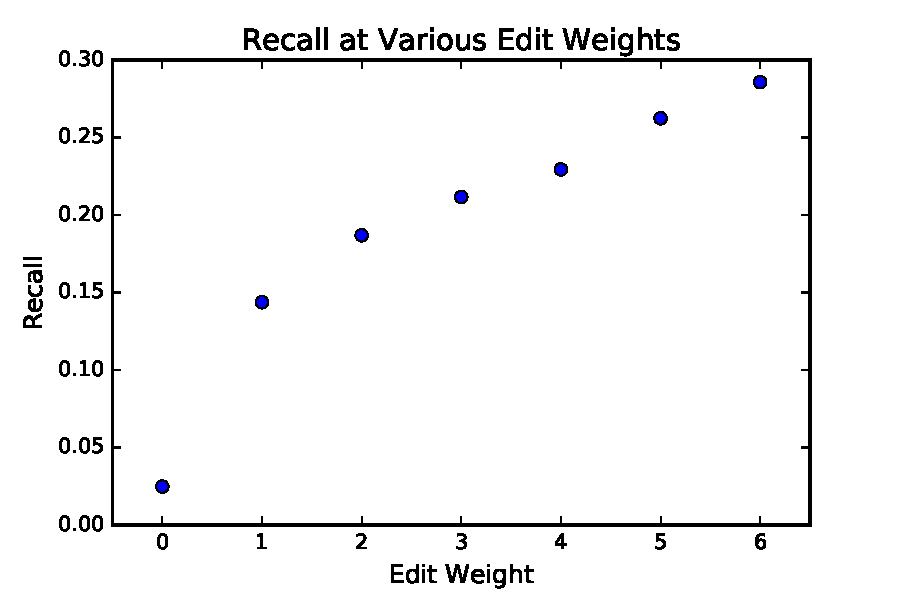
\includegraphics[]{edit_weight_recall}
\caption{The greater the edit weight, the greater the recall.}
\label{fig:edit-weight-recall}
\end{figure}

\begin{figure}[h]
\centering
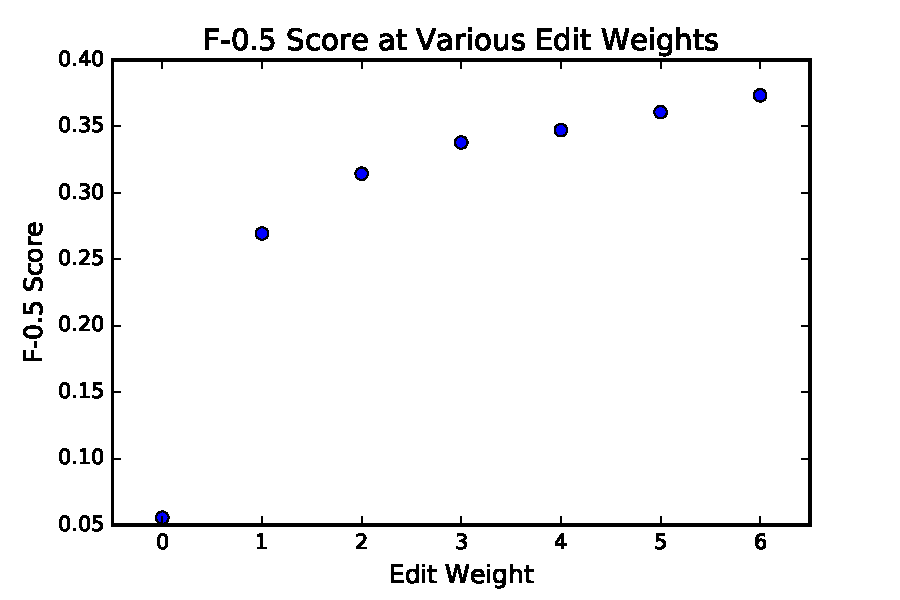
\includegraphics[]{edit_weight_F-0_5}
\caption{Generally speaking, $F_{0.5}$ score also increases with edit weight.}
\label{fig:edit-weight-m2}
\end{figure}
\chapter{Conclusion} \label{ch:conclusion}
The results of this project have shown that applying an edit-based weighted cost function in training a neural machine translation framework for grammatical error correction can make learning more effective. Specifically, emphasising edit words more than non-edit words enforces that the system learn to actually correct grammatical errors instead of simply copying text. The result is greater recall and $F$ score with no compromise to precision.

To take these results further, we suggest training deeper models and varying training hyperparameters.
%% ... etc ...

%%%%%%%%
%% Any appendices should go here. The appendix files should look just like the
%% chapter files.
\appendix
\include{appendix1}
%% ... etc...

%% Choose your favourite bibliography style here.
\bibliographystyle{apalike}

%% If you want the bibliography single-spaced (which is allowed), uncomment
%% the next line.
% \singlespace

%% Specify the bibliography file. Default is thesis.bib.
\bibliography{thesis,books}

%% ... that's all, folks!
\end{document}
